\documentclass{beamer}

\usetheme[language=italian,
		  bullet=triangle,
		  color=green,
		  titleline=true,
		  notshowauthor=true,
		  notshowtitle=true
         ]{TorinoTh}
\setbeamertemplate{caption}[numbered] % per avere fig. numerate nelle caption
\makeatletter
\renewcommand{\fnum@figure}{Fig. \thefigure} %per avere fig. invece che figura
\makeatother
\usepackage[beamer,customcolors]{hf-tikz}
\usepackage{graphicx}
\usepackage[font={footnotesize}]{caption}
\usepackage{wrapfig}
\hfsetfillcolor{alerted text.fg!10}
\hfsetbordercolor{alerted text.fg}

\begin{center}
\small Alma Mater Studiorum - Università di Bologna
\end{center}
\begin{center}
\small Scuola di Scienze - Corso di Laurea in Informatica
\end{center}

\author{Giulia Cantini}
\rel{Renzo Davoli}
\title{Studio e sperimentazione di strumenti software per presentazioni pubbliche basati su Raspberry Pi}
\ateneo{Università di Bologna}

%\date{Sessione II\\
%Anno Accademico 2016/2017\\ \\
%11 ottobre 2017} lo voglio fare uguale al frontespizio della tesi TODO

\date{11 ottobre 2017}

\begin{document}

\titlepageframe % Specific command

\begin{frame}[fragile]{Introduzione}

\begin{itemize}
    \item I proiettori wireless sono utilizzati in molti ambiti diversi (aziende, eventi pubblici, privati) spesso come sostituti dei modelli cablati, rispetto ai quali offrono alcuni vantaggi
    \item Non esiste uno standard ma esistono tecnologie wireless diverse, la tecnologia scelta caratterizza il funzionamento del proiettore determinandone pregi e limitazioni
    \item Tra i difetti presenti vi sono le restrizioni sui tipi di file che possono essere trasmessi, le modalità di connessione e i costi elevati
    \item La soluzione qui proposta - basata sull'utilizzo di VNC e Raspberry Pi - si presenta come alternativa alle precedenti.
\end{itemize}
\end{frame}


\begin{frame}[fragile]{Tecnologie e strumenti}

\begin{columns}[T]
\begin{column}{.25\textwidth}
\newline
\begin{itemize}
  \setlength\itemsep{4em}
  \newline
    \item VNC \newline
    \highlightbf{V}irtual\newline
    \highlightbf{N}etwork\newline
    \highlightbf{C}omputing\newline
    \item Raspberry Pi\newline
\end{itemize}

\end{column}%
\hfill%
\begin{column}{.60\textwidth}
    \begin{figure}[t!]
    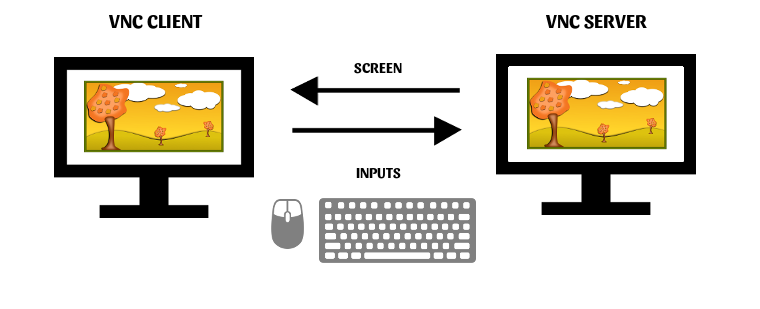
\includegraphics[scale=2.0]{../img/vnc-client-server-cut.png}
    \caption{Interazione tra un client e un server VNC}
%\begin{figure}[!htb]
%\minipage{0.49\textwidth}
%\centering
%  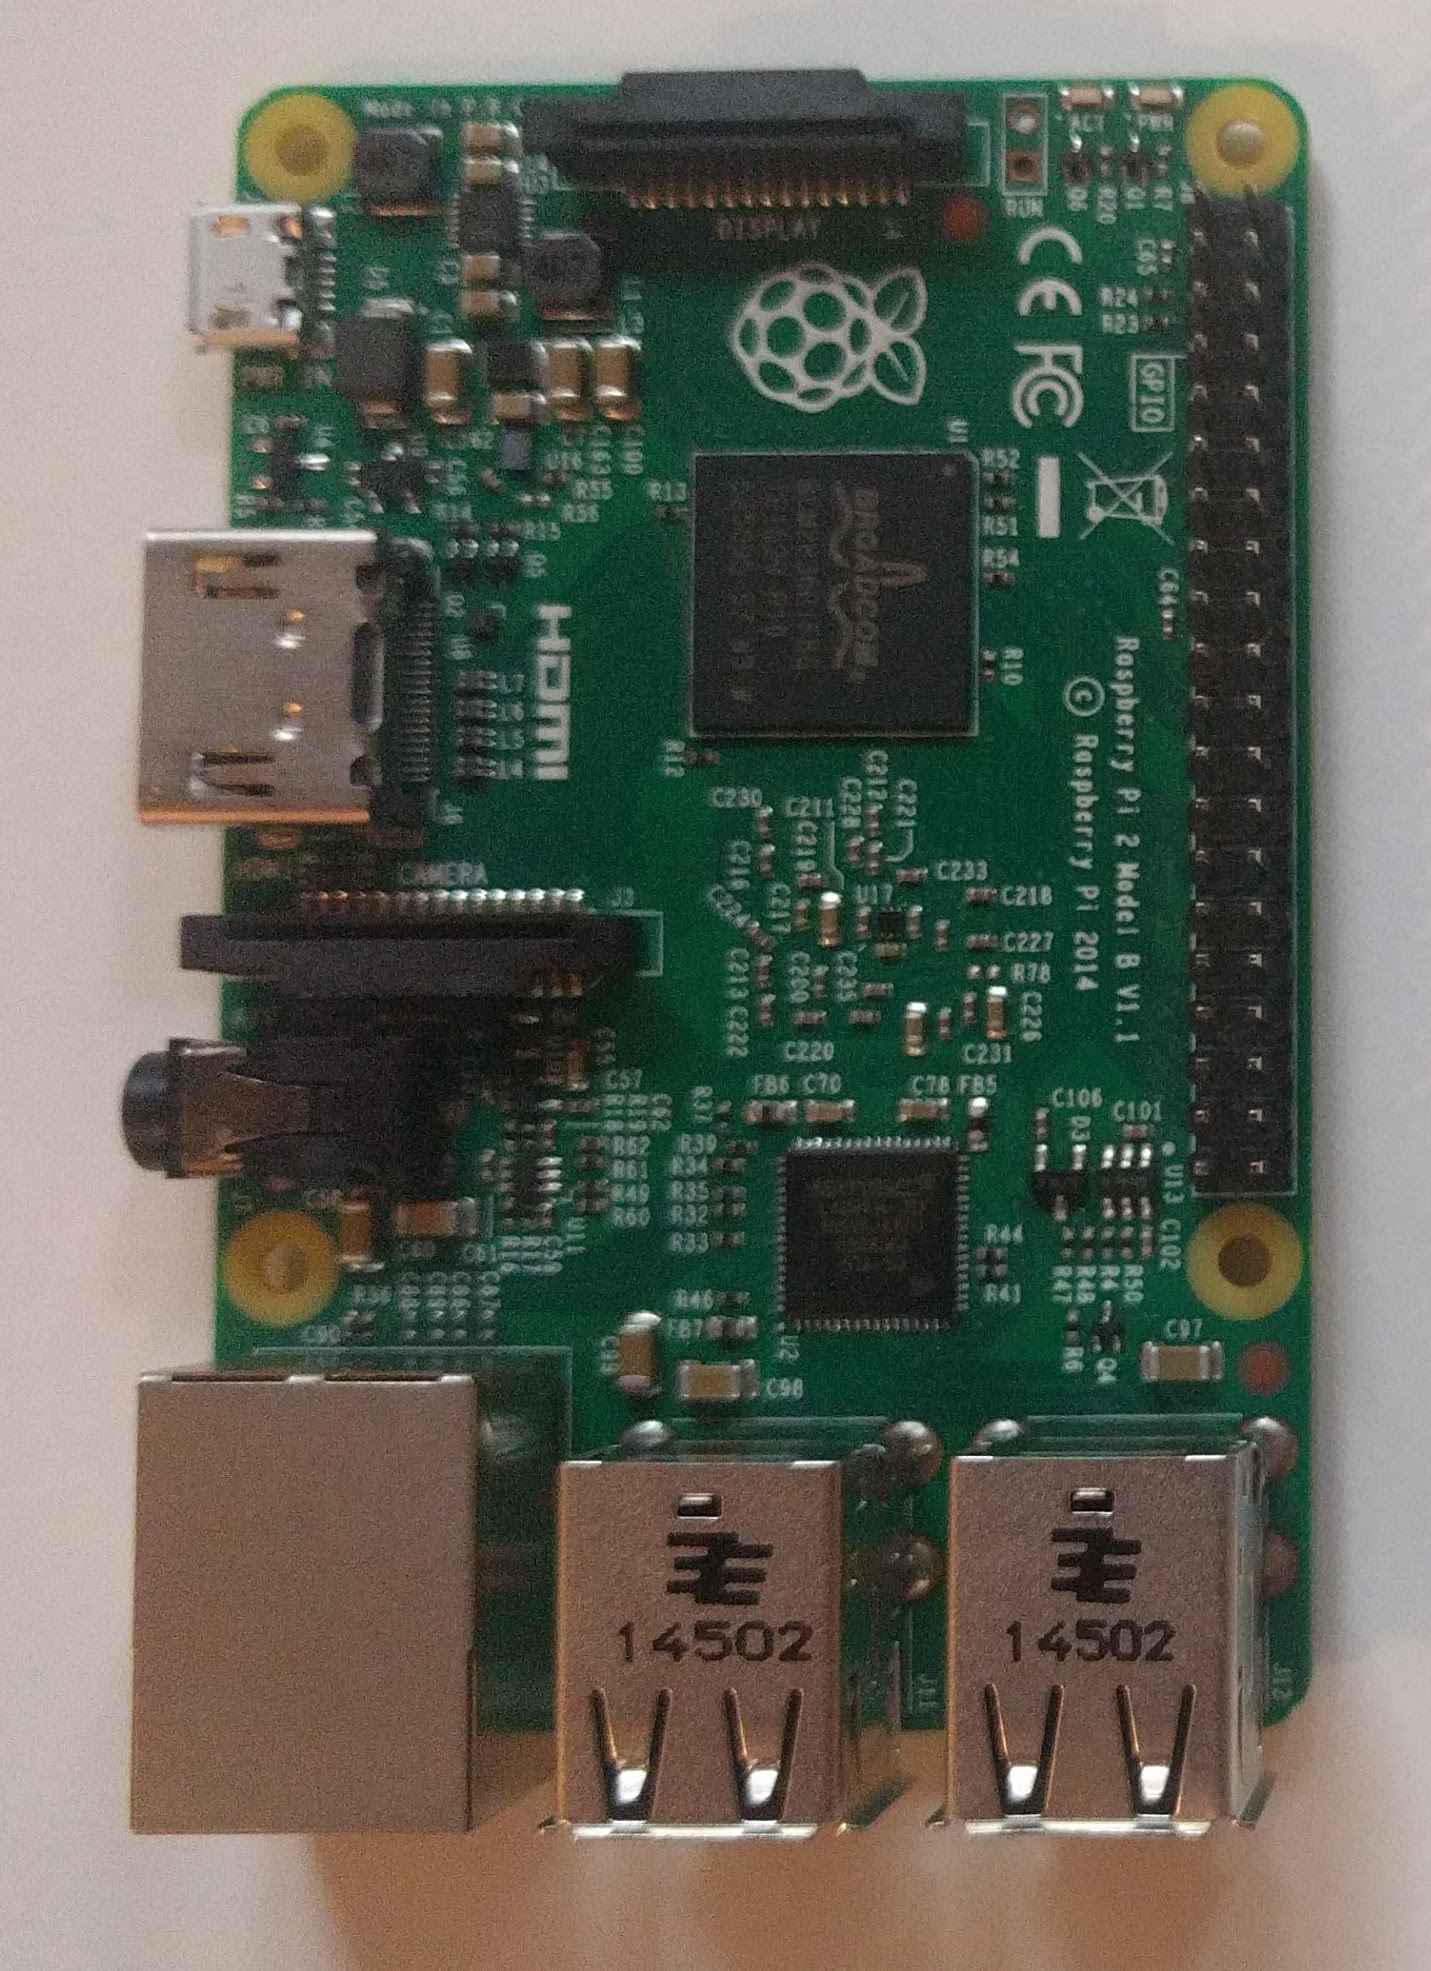
\includegraphics[width=0.5\linewidth]{../img/pi2.jpg}
%  \caption{A really Awesome Image}\label{fig:awesome_image1}
%\endminipage\hfill
%\minipage{0.49\textwidth}
%\centering
%  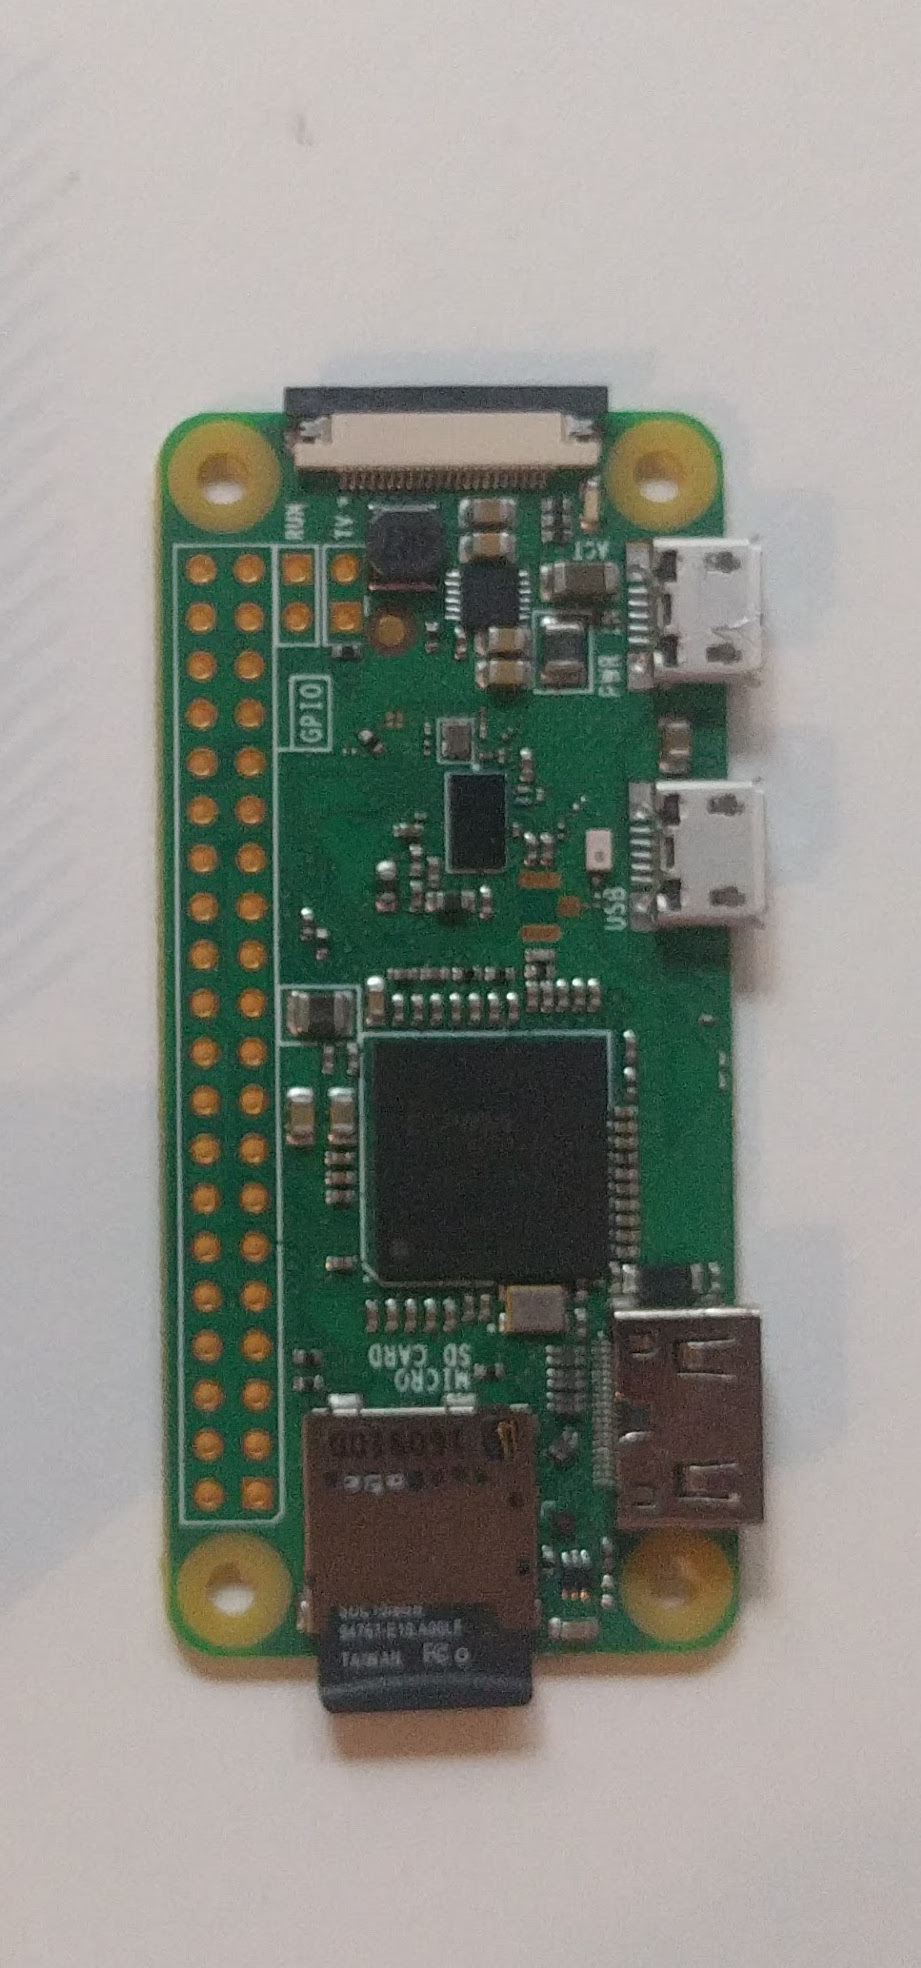
\includegraphics[width=0.3\linewidth]{../img/pizero.jpg}
%  \caption{\small{A really Awesome Image}}\label{fig:awesome_image2}
%\endminipage
%\end{figure}
    \centering
    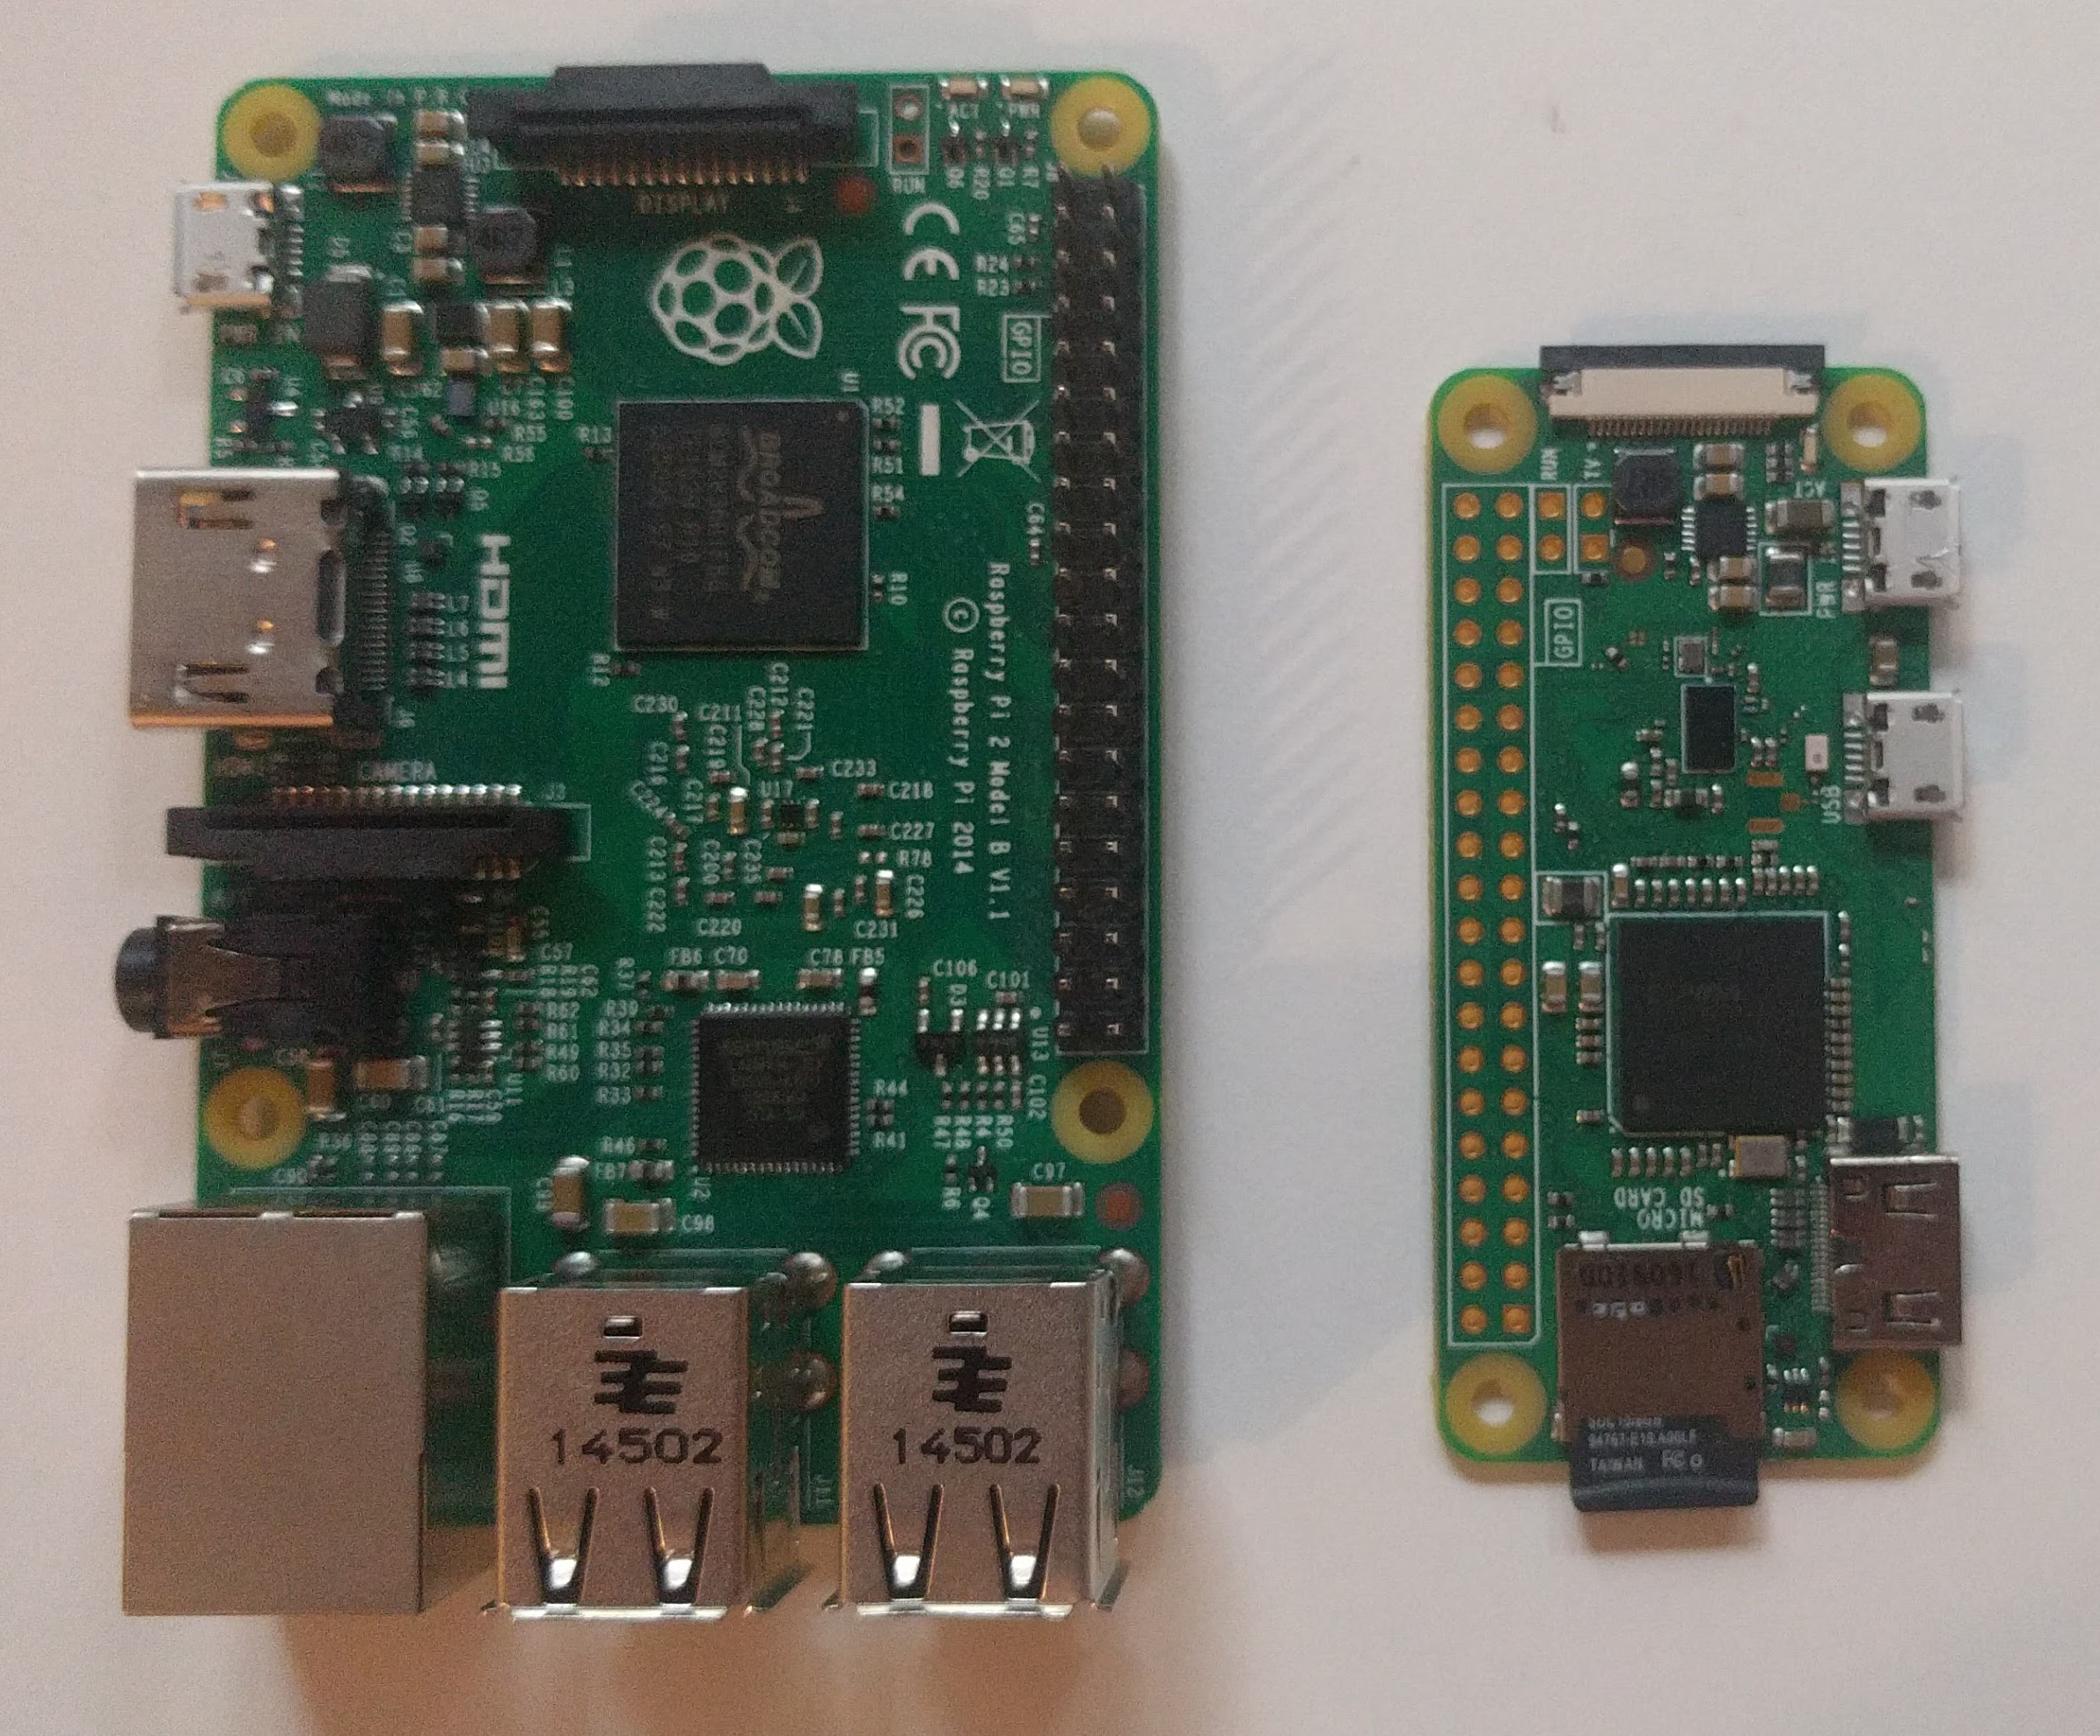
\includegraphics[scale=0.03]{../img/pi-comparison.jpg}
    \caption{Raspberry Pi 2 e Raspberry Pi Zero W.}
\end{figure}
\end{column}%non mi piacciono le immagini
\end{columns}
\end{frame}

\begin{frame}[fragile]{Raspberry Pi Wireless Projector}

\begin{columns}[T]
    \begin{column}{.37\textwidth}
    Il sistema è formato da un proiettore tradizionale collegato via cavo ad un Raspberry Pi (client VNC), connesso a sua volta ad un laptop (server VNC).


    \vspace{1em}
    Il collegamento VNC è stabilito tramite un meccanismo chiamato \emph{reverse connection}.

    \end{column}
    \begin{column}{.61\textwidth}
    \begin{figure}
        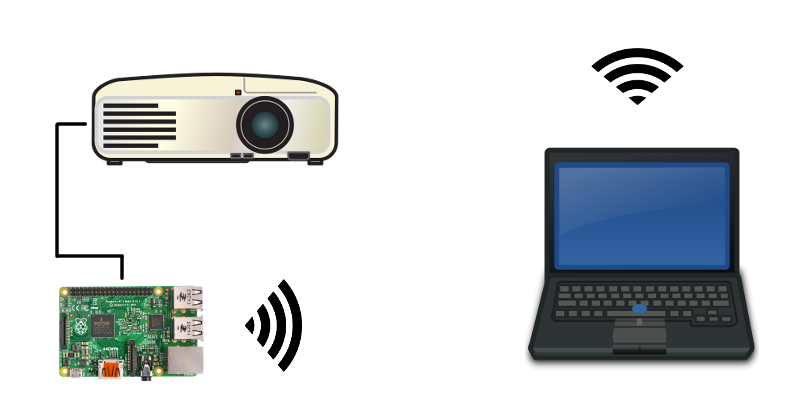
\includegraphics[scale=1.9]{../img/setup.png}
        \caption{Panoramica del sistema.}
    \end{figure}
    \end{column}
\end{columns}
\end{frame}

\begin{frame}[fragile]{Configurazione del server}

È necessario differenziare in base al sistema operativo:\newline
\begin{itemize}
    \item Windows (TightVNC)
    \item macOS (Vine Server/OSXvnc)
    \item GNU/Linux (x11vnc)

\end{itemize}

\begin{itemize}
    \item hostname
    \item modifica della risoluzione
    \item riduzione della parte di schermo da condividere
\end{itemize}
\end{frame}

\begin{frame}[fragile]{Configurazione del client (1)}
 \begin{itemize}
    \setlength\itemsep{2em}
     \item Startup\newline
     il client VNC viene eseguito in automatico all'avvio tramite creazione di desktop entry

     \item Indirizzo IP statico\newline
     viene abilitato modificando il file di configurazione del demone dhcpcd
     \item Blank screen\newline
     viene disabilitato agendo sul file di configurazione di LightDM, il display manager
 \end{itemize}

 %%TODO magari dividere in due colonne e a dx mettere i listings...
\end{frame}

\begin{frame}[fragile]{Configurazione del client (2)}
 \begin{itemize}
   \setlength\itemsep{2em}
     \item Streaming audio e video
     \vspace{0.5em}
        \begin{itemize}
           \setlength\itemsep{0.5em}
        \item PulseAudio
        \end{itemize}
     \item File system read-only
     \vspace{0.5em}
        \begin{itemize}
        \setlength\itemsep{0.5em}
        \item Motivazioni
        \item Tabella delle partizioni
        \item UnionFS
        \item Abilitare temporaneamente la lettura-scrittura
        \end{itemize}

 \end{itemize}
\end{frame}

\begin{frame}[fragile]{VNC on the GO}

\begin{columns}[T]
    \begin{column}{.37\textwidth}
    \begin{itemize}
    \item Uso wireless\newline
    \small come estensione del Raspberry Pi Wireless Projector
    \item \normalsize Uso wired\newline
    \small in caso di disponibilità di soli proiettori tradizionali\\
    \end{itemize}

    \end{column}
    \begin{column}{.61\textwidth}
    \begin{figure}
        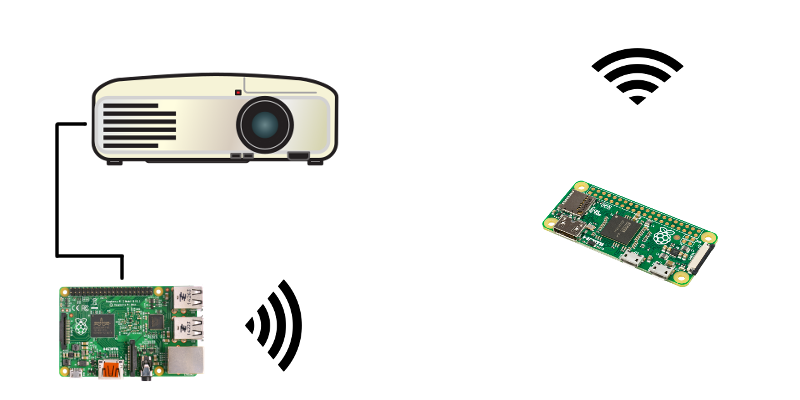
\includegraphics[scale=1.5]{../img/setup-with-pizero.png}
        \caption{Uso wireless.}
    \end{figure}
    \end{column}
\end{columns}
\vspace{1em}

 La configurazione del sistema si basa sulla presenza di una directory predefinita che contiene le presentazioni e uno script che esegue all'avvio tramite file .desktop i programmi necessari per la presentazione: VNC (per uso wireless), Piremote, Evince.
\end{frame}

\begin{frame}[fragile]{Piremote}

\begin{columns}[T]
    \begin{column}{.48\textwidth}
    Disponibile a http://github.com/giulic3/piremote.

    \vspace{1em}
    Consente lo scorrimento delle pagine nella presentazione corrente, la navigazione all'interno della directory principale e l'apertura di nuove presentazioni.

    \end{column}
    \begin{column}{.48\textwidth}
    \begin{figure}
        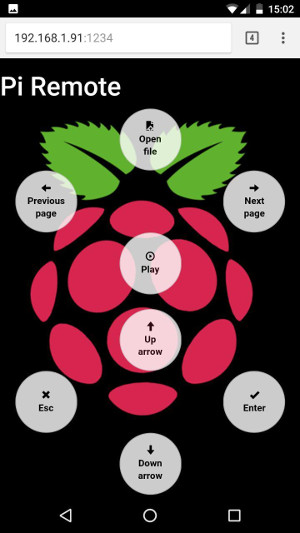
\includegraphics[scale=0.41]{../img/main_page.jpg}
        \caption{Pagina di controllo di Piremote}
    \end{figure}
    \end{column}
\end{columns}
\end{frame}

\begin{frame}[fragile]{Conclusioni e sviluppi futuri}
 \begin{itemize}
     \item Estensione del supporto server per dispositivi mobili (Android/iOS)
     \item Stabilità del canale nello streaming audio
     \item Tempi di avvio del Raspberry Pi Zero W
     \item Tempi di risposta in VNC on the GO
     \item Modalità di caricamento delle presentazioni
     \item Estensione delle possibilità di controllo tramite Piremote

 \end{itemize}
\end{frame}

\begin{frame}[c]

\begin{center}
\LARGE Grazie per l'attenzione
\end{center}
\end{frame}

\begin{frame}[plain, noframenumbering]{Approfondimento: Limitazioni dei proiettori wireless}

Riguardano:\newline

\begin{itemize}

\item La tipologia di file trasmessi, con la mancanza di supporto video o risultati non soddisfacenti nella riproduzione
\item Le modalità di connessione, quando il servizio non è integrato in una rete esistente ma è richiesta la creazione di una rete ad hoc
\item Hardware aggiuntivo (es. adattatori USB) necessario per il funzionamento
\item I costi elevati, con differenze tra proiettori con WiFi built-in e proiettori tradizionali potenziati da adattatori wireless.

\end{itemize}
\end{frame}



\begin{frame}[plain, noframenumbering]{Approfondimento: File system e UnionFS}

\begin{itemize}
\item Tipo di file system che supporta union mount
\item È utilizzato per sovrapporre ad un sistema in sola lettura, un file system temporaneo memorizzato in RAM
\item Di conseguenza ogni scrittura avviene in RAM e verrà persa ad ogni riavvio, evitando potenziali scritture dannose su memoria SD.
\end{itemize}
\end{frame}

\begin{frame}[plain, noframenumbering]{Approfondimento: Piremote}

\begin{itemize}

\item Realizzato in Python, Javascript per il frontend
\item È basato su un modulo che consente il controllo completo di mouse e tastiera
\item Piremote può essere eseguito da riga di comando eventualmente specificando i parametri \textit{address}, \textit{port}, \textit{key}.

\end{itemize}

\end{frame}




\end{document}
